\section{Experiments}\label{sec:exp}
\label{sec:experiments}

We conduct experiments to evaluate \algname{} and to understand when online harness evolution improves LLM agents:
\begin{itemize}[leftmargin=12pt,noitemsep,topsep=2pt]
    \item \textbf{RQ1: Overall effectiveness.}
    Does \algname{} improve frozen agents across diverse benchmarks, and which task categories benefit most?
    \item \textbf{RQ2: Harness content and components.}
    What types of guidance are produced by the evolved harness, and how do different harness components contribute?
    \item \textbf{RQ3: Online updating and transfer.}
    How do evolved harnesses behave under train-split transfer, online updating, and solver-evolver pairing?
    \item \textbf{RQ4: Feedback grounding.}
    How does the source and granularity of feedback affect harness evolution?
\end{itemize}

\subsection{Setup}\label{sec:exp-setup}

\mypara{Experimental setup.}
We evaluate \algname{} on five benchmarks spanning diverse agent capabilities: WebArena-Infinity~\citep{zhou2026wainf} for web navigation, TerminalBench2~\citep{merrill2026terminalbenchbenchmarkingagentshard} for command-line tasks, SWE-bench Lite~\citep{jimenez2024swebench} for software engineering, CL-Bench~\citep{dou2026cl} for adaptive reasoning, and TAU-Bench~\citep{yao2024tau} for tool-use tasks. We use Claude Opus 4.6 \cite{claude_opus_46} as the default solver and evolver, and additionally evaluate with Claude Opus 4.7 \cite{claude_opus_47}, Claude Opus 4.5 \cite{claude_opus_45}, Kimi-K2.5 \cite{team2026kimi}, and GPT-OSS \cite{agarwal2025gpt} when studying model ablations. We report success rates in percent, where higher is better. Further benchmark and implementation details are provided in Appendix~\ref{app:benchmarks} and \ref{app:details}.

\mypara{Baselines.}
We compare with representative experience-, memory-, and skill-based adaptation methods under the same task split and evaluation protocol. AWM~\citep{wang2024agent} reuses agent working memory, Dynamic Cheatsheet~\citep{suzgun2025dynamic} maintains an adaptive external cheatsheet, Evo-Memory~\citep{wei2025evo} evolves reusable memories from executions, ACE~\citep{zhang2025agentic} optimizes agent context, and XSkill~\citep{jiang2026xskill} separates experience and skills for continual reuse. DC-Cu and DC-RS are two Dynamic Cheatsheet variants.

% \tingwei{just curious, since we are in an sequential setting (and previous learned harness will impact latter tasks), does the ordering of the tasks in each dataset during eval matter? do we have a specific order or they are just random?}

\begin{figure}
    \centering
    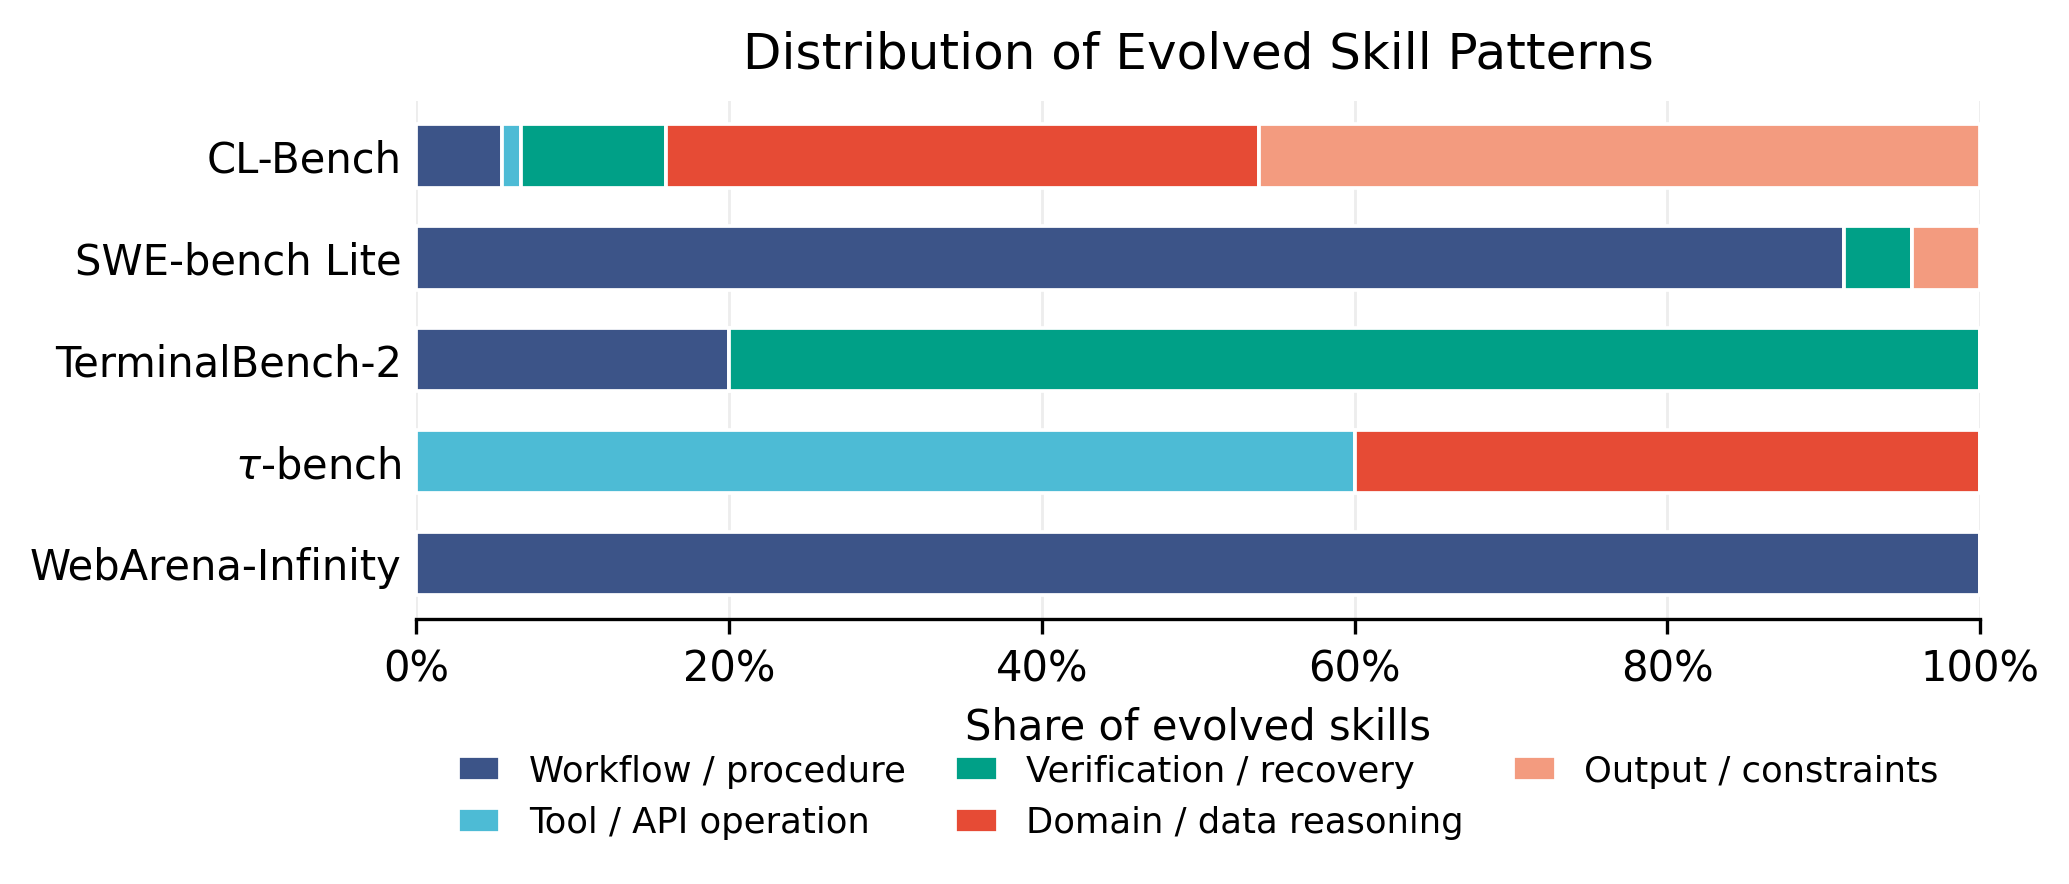
\includegraphics[width=\linewidth]{figures/skill_taxonomy_general.png}
    \caption{Distribution of evolved skill patterns across benchmarks. The learned skills exhibit benchmark-specific characteristics, ranging from workflow and tool-use procedures to verification, domain reasoning, and output-constraint handling.}    
    \label{fig:skill-taxonomy}
\end{figure}

\begin{table*}[t]
\caption{
Main results using Claude Opus 4.6 as the solver. Scores denote success rates (\%), and higher values indicate better performance. \algname{} achieves the best results across all five benchmarks.
}
\centering
\label{tab:main}
\small
\begin{tabular}{lccccc}
\toprule
\textbf{Method} & \textbf{CL-Bench} & \textbf{TerminalBench-2} & \textbf{SWE-bench Lite} & \textbf{$\tau$-bench} & \textbf{WebArena-Infinity} \\
\midrule
No Evolve & 29.54 & 62.92 & 63.67 & 72.73 & 72.50 \\
\midrule
AWM & 28.91 & 62.92 & 62.67 & 70.91 & 70.00 \\
DC-Cu & 29.23 & 60.67 & 63.00 & 72.12 & 71.25 \\
DC-RS & 29.07 & 61.80 & 61.67 & 70.91 & 70.00 \\
Evo-Memory & 29.38 & 64.04 & 64.00 & 72.12 & 72.50 \\
ACE & 29.70 & 61.80 & 63.67 & 72.73 & 71.25 \\
XSkill & 31.44 & 66.29 & 64.67 & 73.94 & 73.75 \\
\midrule
\algname{} & \textbf{34.02} & \textbf{73.03} & \textbf{67.00} & \textbf{76.97} & \textbf{76.25} \\
\bottomrule
\end{tabular}
\label{tab:main-opus46}
\end{table*}

\subsection{Overall Effectiveness (RQ1)}
\label{sec:exp-main}

Table~\ref{tab:main} reports the main results with Claude Opus 4.6 as the solver. 
\textbf{\algname{} improves over both No-Evolve and prior experience-based baselines across all five benchmarks.}
The gains are especially large on TerminalBench-2, where agents need to inspect files, execute commands, interpret errors, and recover from failed operations. This suggests that harness evolution is particularly useful when tasks expose reusable procedural structure.

Compared with the strongest baseline, XSkill, \algname{} still improves on every benchmark. 
\textbf{External experience reuse is not automatically beneficial.}
Several baselines underperform No-Evolve on some benchmarks, suggesting that retrieved or evolved guidance can be noisy, overly specific, or mismatched to the solver. This supports our motivation for studying not only whether self-evolution helps, but also what factors make online harness updates effective.

\subsection{Category and Model Generality (RQ1)}
\label{sec:exp-category-model}

Table~\ref{tab:clbench-category} provides a representative category-level view on CL-Bench across five solver models. Since CL-Bench covers diverse reasoning and execution categories, it allows us to examine where harness evolution is most effective and how the effect varies across solver capabilities.
\textbf{\algname{} improves the overall score for every solver model, with larger gains on stronger Claude models than on open-weight alternatives.}
Opus 4.7, Opus 4.6, and Opus 4.5 obtain gains of $+3.7$, $+4.5$, and $+3.8$, respectively, while Kimi-K2.5 and GPT-OSS improve by $+1.1$ and $+0.8$. This suggests that stronger solvers may be better able to interpret, follow, and benefit from evolved harness guidance.

Across categories, the most consistent improvements appear on Procedural Task Execution (PTE), where every model improves and Opus 4.6 and Opus 4.5 each gain $+9.8$ points. 
\textbf{Harness evolution is most reliable when tasks expose reusable operational structure.}
In contrast, Empirical Discovery \& Simulation (EDS) shows less stable gains, with drops for Opus 4.6 and GPT-OSS. This suggests that more exploratory tasks may be more sensitive to overly specific guidance.






\begin{table*}[t]
\centering
\caption{CL-Bench category results across different models: pass rate (\%) across five models. \textbf{Bold} = best per category-model pair. $\Delta$ shows absolute improvement of \algname{} over the No-Evolve baseline. DKR = Domain Knowledge Reasoning, EDS = Empirical Discovery \& Simulation, PTE = Procedural Task Execution, RSA = Rule System Application.}
\label{tab:clbench-category}
\vspace{3pt}
\small
\setlength{\tabcolsep}{4pt}
\begin{tabular}{ll|cc|cc|cc|cc|cc}
\toprule
& & \multicolumn{2}{c|}{\textbf{DKR}} & \multicolumn{2}{c|}{\textbf{EDS}} & \multicolumn{2}{c|}{\textbf{PTE}} & \multicolumn{2}{c|}{\textbf{RSA}} & \multicolumn{2}{c}{\textbf{All}} \\
\textbf{Model} & \textbf{Method} & Rate & $\Delta$ & Rate & $\Delta$ & Rate & $\Delta$ & Rate & $\Delta$ & Rate & $\Delta$ \\
\midrule
\multirow{2}{*}{Opus 4.7}
& No-Evolve & 32.4 & --- & \textbf{19.1} & --- & 35.5 & --- & 29.0 & --- & 30.8 & --- \\
& \algname{} & \textbf{34.1} & \gain{1.7} & 19.6 & \gain{0.5} & \textbf{42.7} & \gain{7.2} & \textbf{32.7} & \gain{3.7} & \textbf{34.5} & \gain{3.7} \\
\midrule
\multirow{2}{*}{Opus 4.6}
& No-Evolve & 31.4 & --- & \textbf{20.6} & --- & 34.0 & --- & 26.9 & --- & 29.5 & --- \\
& \algname{} & \textbf{35.6} & \gain{4.2} & 18.1 & \loss{-2.5} & \textbf{43.8} & \gain{9.8} & \textbf{30.4} & \gain{3.5} & \textbf{34.0} & \gain{4.5} \\
\midrule
\multirow{2}{*}{Opus 4.5}
& No-Evolve & 31.4 & --- & 18.1 & --- & 27.8 & --- & 25.3 & --- & 27.3 & --- \\
& \algname{} & \textbf{32.6} & \gain{1.2} & \textbf{19.1} & \gain{1.0} & \textbf{37.6} & \gain{9.8} & \textbf{28.3} & \gain{3.0} & \textbf{31.1} & \gain{3.8} \\
\midrule
\multirow{2}{*}{Kimi-K2.5}
& No-Evolve & 25.6 & --- & 12.1 & --- & 25.1 & --- & \textbf{21.6} & --- & 22.9 & --- \\
& \algname{} & \textbf{25.9} & \gain{0.3} & \textbf{13.1} & \gain{1.0} & \textbf{29.3} & \gain{4.2} & 20.8 & \loss{-0.7} & \textbf{23.9} & \gain{1.1} \\
\midrule
\multirow{2}{*}{GPT-OSS}
& No-Evolve & 17.6 & --- & \textbf{11.6} & --- & 17.6 & --- & 16.4 & --- & 16.6 & --- \\
& \algname{} & \textbf{17.9} & \gain{0.3} & 10.6 & \loss{-1.0} & \textbf{18.5} & \gain{0.8} & \textbf{18.6} & \gain{2.1} & \textbf{17.5} & \gain{0.8} \\
\bottomrule
\end{tabular}
\vspace{-5pt}
\end{table*}


\begin{table}[t]
\centering
\caption{Ablation study on CL-Bench and SWE-bench Lite using Claude Opus 4.6 as the solver. Scores denote pass rates (\%).}
\label{tab:ablation-cl-swe}
\vspace{3pt}
\small
\begin{tabular}{lcc}
\toprule
\textbf{Method} & \textbf{CL-Bench} & \textbf{SWE-bench Lite} \\
\midrule
No Evolve & 29.54 & 63.67 \\ \midrule
No Propose & 33.28 & 65.33 \\
General Only & 30.28 & 66.67 \\
Topic Only & 33.70 & 64.33 \\
\midrule
\algname{} & \textbf{34.02} & \textbf{67.00} \\
\bottomrule
\end{tabular}
\vspace{-5pt}
\end{table}

\subsection{Harness Content and Components (RQ2)}
\label{sec:exp-harness-analysis}

% Figure~\ref{fig:skill-taxonomy} analyzes the content of the evolved harness across benchmarks. 
% \textbf{The evolved harness reflects benchmark-specific operational demands rather than accumulating generic guidance.} WebArena-Infinity is dominated by workflow and procedure skills, which is consistent with interface-driven tasks that require multi-step navigation and state manipulation. TerminalBench-2 contains a large share of verification and recovery skills, reflecting the need to inspect command outputs, diagnose failures, and validate intermediate states. $\tau$-bench contains a mixture of tool/API operation and domain/data reasoning skills, matching its structured tool-use setting. CL-Bench shows a broader distribution, including domain reasoning and output-constraint handling, which is consistent with its adaptive reasoning tasks. These patterns support our view that context-to-harness compilation adapts the harness to the operational structure and failure modes of each environment.

Figure~\ref{fig:skill-taxonomy} analyzes the content of the evolved harness across benchmarks. 
\textbf{The evolved harness reflects benchmark-specific operational demands rather than accumulating generic guidance.}
WebArena-Infinity mainly yields workflow and procedure skills, TerminalBench-2 emphasizes verification and recovery, $\tau$-bench mixes tool/API operation with domain reasoning, and CL-Bench produces a broader distribution including domain reasoning and output-constraint handling. These patterns suggest that context-to-harness compilation adapts the harness to each environment's operational structure and failure modes.



Table~\ref{tab:ablation-cl-swe} studies which parts of the harness update process contribute to performance. We focus this and the following diagnostic analyses mainly on CL-Bench and SWE-bench Lite because they stress different forms of harness guidance: CL-Bench contains heterogeneous adaptive reasoning tasks where localized task-type guidance can matter, while SWE-bench Lite emphasizes repository-level debugging and verification procedures where broader reusable guidance is expected to help. \textsc{No Propose} removes solver-side proposal of candidate memories, \textsc{General Only} keeps only cross-task guidance, and \textsc{Topic Only} keeps only localized task-type guidance.

% \textbf{Both broad cross-task guidance and localized task-type guidance are useful, but their importance depends on the task setting.}
% The full \algname{} setting achieves the best performance on both benchmarks, reaching $34.02$ on CL-Bench and $67.00$ on SWE-bench Lite. On CL-Bench, Topic Only reaches $33.70$, close to the full method, while General Only reaches $30.28$, suggesting that CL-Bench benefits from localized operational knowledge associated with recurring task types or contexts. On SWE-bench Lite, the pattern is reversed: General Only reaches $66.67$, close to the full method, while Topic Only reaches $64.33$, suggesting that SWE-bench Lite benefits more from broad procedures such as repository inspection, debugging, verification, and test-driven repair. No Propose improves over No Evolve on both benchmarks but remains below the full method, indicating that proposal and harness-level compilation are complementary.

\textbf{Both broad cross-task guidance and localized task-type guidance are useful, but their importance depends on the task setting.}
The full \algname{} setting performs best on both benchmarks. On CL-Bench, Topic Only reaches $33.70$, close to the full result of $34.02$, while General Only drops to $30.28$, suggesting that localized task-type guidance is more useful for its heterogeneous reasoning tasks. On SWE-bench Lite, General Only reaches $66.67$, close to the full result of $67.00$, while Topic Only reaches $64.33$, indicating that broad debugging, verification, and repository-inspection procedures matter more. No Propose improves over No Evolve but remains below the full method, suggesting that proposal and harness-level compilation are complementary.



\begin{figure}
    \centering
    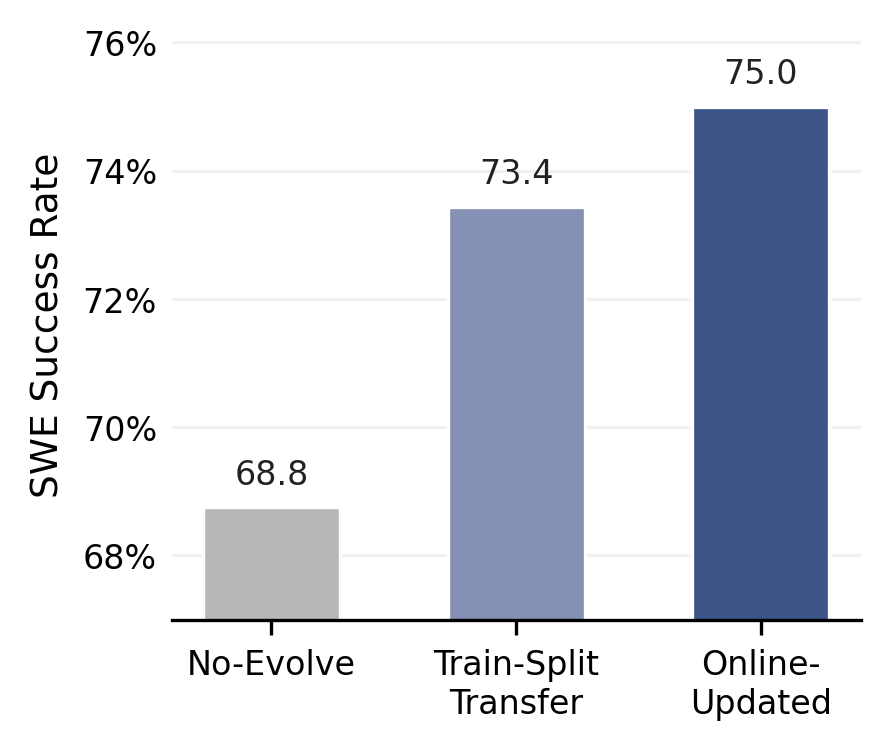
\includegraphics[width=0.7\linewidth]{figures/swe_cross_skill_transfer.png}
\caption{SWE-bench Lite success rates under different evolution settings. 
\textsc{No-Evolve} uses no harness updates; \textsc{Train-Split Transfer} evaluates skills evolved by Claude Sonnet on the training split; and \textsc{Online-Updated} updates skills during the task stream. }
    \label{fig:swe-evolution-setting}
    \vspace{-0.5cm}
\end{figure}

% ===========================================================================
\subsection{Transfer and Adaptability (RQ3)}
\label{sec:exp-transfer}
% ===========================================================================



Figure~\ref{fig:swe-evolution-setting} compares three skill-update settings. \textsc{No-Evolve} uses no harness update. \textsc{Train-Split Transfer} uses skills evolved by Claude Sonnet 4.5 on the training split and evaluates them with an Opus 4.7 solver on the test split. \textsc{Online-Updated} updates the harness directly with the same models during the test task stream. 
\textbf{Skills learned on a training split can transfer across both tasks and models, while online updating performs best.}
No-Evolve reaches $68.8$, Train-Split Transfer reaches $73.4$, and Online-Updated reaches $75.0$. The gain from Train-Split Transfer shows that skills evolved by a smaller or different model can still provide useful guidance for a stronger solver on unseen tasks. Online-Updated further improves over Train-Split Transfer by $+1.6$ points, suggesting that in-situ harness updates better adapt to the local distribution and failure modes of the test stream.

Figure~\ref{fig:swe-curator-solver} examines how solver-evolver pairing affects harness evolution. We compare two solver settings: an Opus 4.7 solver and a Sonnet 4.5 solver. In each setting, \textsc{Same} uses the same model as both solver and evolver, while \textsc{Cross} uses the other model as the evolver. Specifically, for the Opus solver, \textsc{Same} uses Opus to evolve the harness and \textsc{Cross} uses Sonnet to evolve the harness; for the Sonnet solver, \textsc{Same} uses Sonnet as the evolver and \textsc{Cross} uses Opus as the evolver.
\textbf{Using the same model for solving and evolution is not always optimal; cross-model evolution can help, but only when the solver is capable of using the evolved guidance.}
For the Opus solver, Cross reaches $76.0$, slightly higher than Same at $75.3$ and clearly above No-Evolve at $70.7$. This suggests that a different evolver can produce guidance that is still useful, or even more useful, when the downstream solver has sufficient capability to interpret and apply it. For the Sonnet solver, however, Same and Cross reach $55.3$ and $55.7$, both below No-Evolve at $58.0$. Thus, Sonnet-evolved skills can help Opus, but do not necessarily help Sonnet itself. This contrast suggests that harness transfer depends not only on the skill artifact but also on the base solver’s capability: if the solver cannot reliably follow, contextualize, or adapt the guidance, evolution may fail to improve performance.

% ===========================================================================
\subsection{Feedback Grounding (RQ4)}
\label{sec:exp-feedback}

% ===========================================================================

\begin{figure}[t]
  \centering
  \begin{subfigure}{0.48\linewidth}
    \centering
    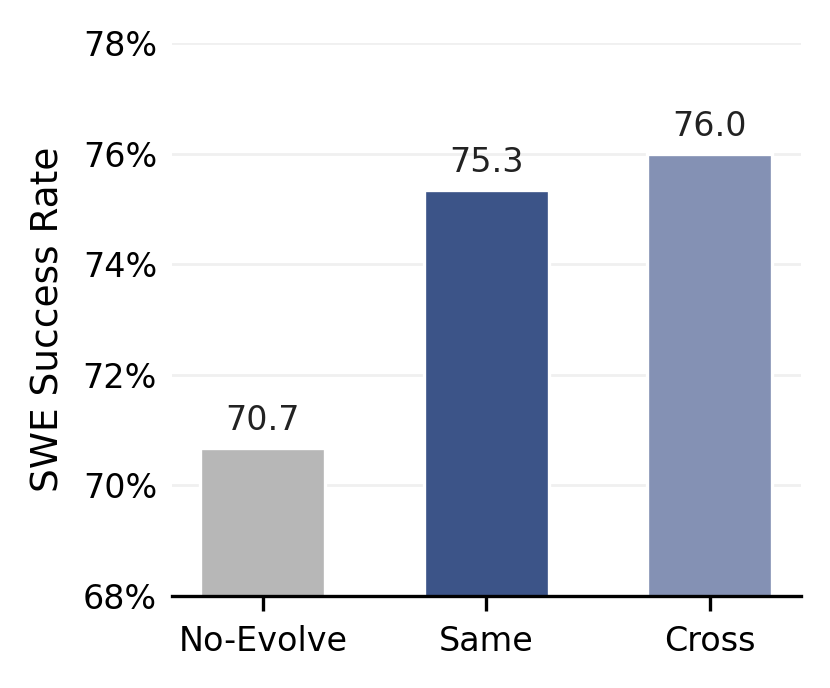
\includegraphics[width=\linewidth]{figures/swe_curator_solver_opus.png}
    \caption{Opus 4.7 Solver}
    \label{fig:swe-curator-opus}
  \end{subfigure}
  \hfill
  \begin{subfigure}{0.48\linewidth}
    \centering
    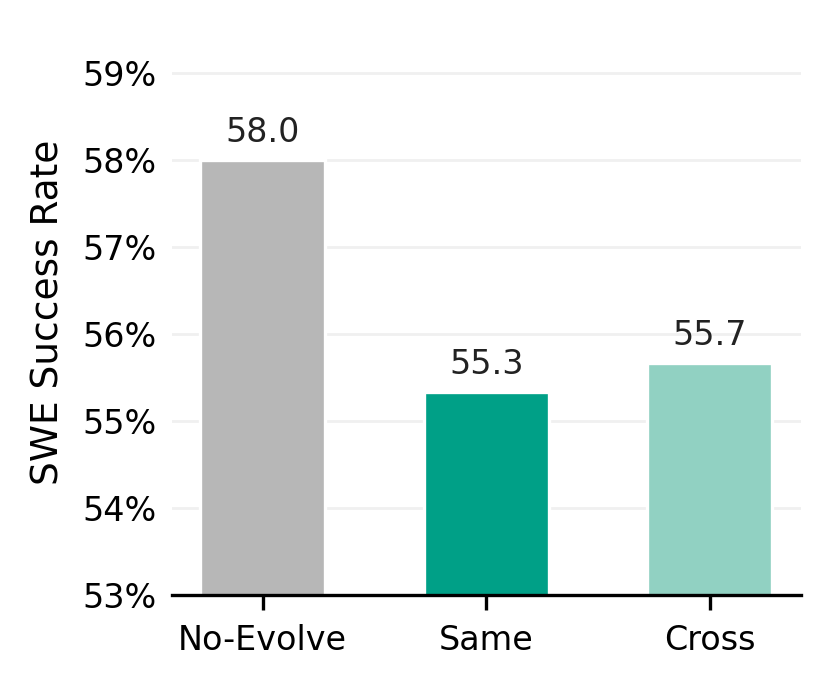
\includegraphics[width=\linewidth]{figures/swe_curator_solver_sonnet.png}
    \caption{Sonnet 4.5 Solver}
    \label{fig:swe-curator-sonnet}
  \end{subfigure}
\caption{Effect of solver-evolver pairing on SWE-bench Lite. 
\textsc{Same} denotes using the same model for solving and skill evolution, while \textsc{Cross} denotes using different models for the solver and evolver. }
  \label{fig:swe-curator-solver}
  \vspace{-0.4cm}
\end{figure}

Table~\ref{tab:feedback-level-ablation} evaluates how feedback signals affect harness evolution on CL-Bench and SWE-bench Lite. We compare three feedback settings. \textsc{Self-Generated} asks the LLM itself to judge whether the execution succeeded and what should be learned. \textsc{Minimal} provides only the environment-level success or failure signal, such as whether a command, verifier, or test passed. \textsc{Standard} provides grounded diagnostic feedback, including failure messages, error traces, verifier outputs, or test failures when available.

\textbf{Grounded feedback is important for reliable harness evolution.}
Self-Generated feedback underperforms No-Evolve on both benchmarks, decreasing CL-Bench from $29.54$ to $27.96$ and SWE-bench Lite from $63.67$ to $61.67$. This suggests that LLM-generated self-judgment can introduce misleading updates when it is not grounded in external execution evidence. In contrast, Minimal and Standard feedback both use environment-provided signals and are more reliable overall.

\textbf{Standard feedback is generally preferable, but the useful granularity of feedback depends on the benchmark.}
On CL-Bench, Standard feedback performs best, reaching $34.02$, while Minimal feedback reaches only $29.86$. This suggests that richer diagnostics are useful for adaptive reasoning tasks, where understanding the reason for failure can help compile better harness guidance. On SWE-bench Lite, however, Minimal feedback reaches $67.33$, slightly above Standard feedback at $67.00$. One possible explanation is that detailed error messages can sometimes make the evolved harness overly tied to task-specific failures, while sparse pass/fail signals encourage more generalizable guidance.



\begin{table}[t]
\centering
\caption{Impact of feedback level on CL-Bench and SWE-bench Lite using Claude Opus 4.6 as the solver. Scores denote pass rates (\%).}
\label{tab:feedback-level-ablation}
\vspace{3pt}
\small
\begin{tabular}{lcc}
\toprule
\textbf{Feedback Level} & \textbf{CL-Bench} & \textbf{SWE-bench Lite} \\
\midrule
No Evolve & 29.54 & 63.67 \\
Self-Generated & 27.96 & 61.67 \\
Minimal & 29.86 & \textbf{67.33} \\
Standard & \textbf{34.02} & 67.00 \\
\bottomrule
\end{tabular}
\vspace{-5pt}
\end{table}






